\section{Граничные обратные задачи и задачи с данными Коши}\label{sec:rev}

\subsection{Граничная обратная задача}\label{subsec:rev}
\begin{frame}
    \frametitle{Граничная обратная задача}
    Модель имеет следующий вид
    \begin{wrapfigure}{r}{0.3\textwidth}
        \centering{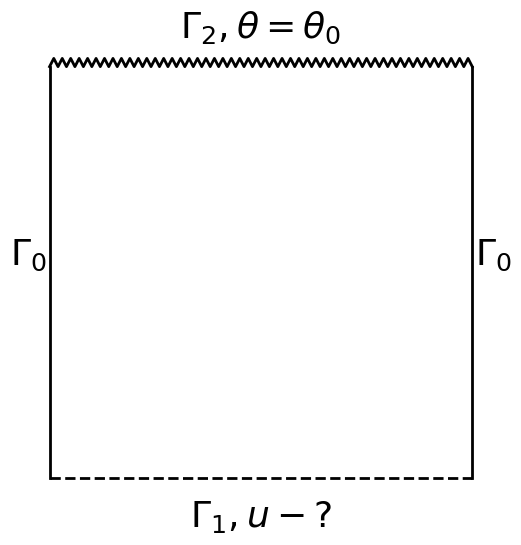
\includegraphics[width=1\linewidth]{omega_1}}
%        \caption*{$\Gamma \coloneqq \partial \Omega =\overline{\Gamma}_0 \cup \overline{\Gamma}_1 \cup \overline{\Gamma}_2$}
    \end{wrapfigure}
    \begin{gather}
        \label{eq:2_1:initial}
        - a \Delta \theta + b \kappa_a(\theta ^ 3 | \theta | - \varphi) = 0, \\
        - \alpha \Delta \varphi + \kappa_a (\varphi - \theta ^3 | \theta |) = 0,
    \end{gather}
    \begin{equation}
        \label{eq:2_1:initial-boundary}
        \begin{aligned}
            \Gamma &: \; a \partial_n \theta + \beta (\theta - \theta _b) = 0, \\
            \Gamma_0 \cup \Gamma_2 &: \; \alpha \partial_n \varphi
            + \gamma(\varphi - \theta_b ^4 ) = 0, \\
            \Gamma_1 &: \; \alpha \partial_n \varphi + u(\varphi - \theta_b ^4 ) = 0. \\
        \end{aligned}
    \end{equation}
    $\Gamma_0, \Gamma_1, \Gamma_2$ не имеют пересечений.

    Функции $\gamma, \theta_b, \beta$ известны.
    \textit{Неизвестная функция $u$ характеризует отражающие свойства участка границы $\Gamma_1$}.
    Предполагается, что $0 < u_1 \leq u \leq u_2$.

    \textbf{Обратная задача} заключается в отыскании тройки $\theta, \varphi, u$
    по дополнительному условию $\theta|_{\Gamma_2} = \theta_0$.

    \textbf{Экстремальная задача} заключается в минимизации функционала
    \begin{equation}
        \label{eq:2_1:quality}
        J(\theta) = \frac{1}{2} \int_{\Gamma_2} (\theta - \theta_0)^2 d\Gamma
    \end{equation}
    на решениях краевой задачи~\eqref{eq:2_1:initial}--\eqref{eq:2_1:initial-boundary}.
\end{frame}
\note{
    \begin{itemize}
        \item Первая из рассматриваемых задач представляется двумя уравнениями ...
        \item Пару $\theta, \varphi$ - будем называть состоянием системы.
        \item Дополняется граничными условиями ...
        \item Если же параметр отражательной способности неизвестен на части границы,но ...
        \item Неизвестные параметры среды мы будем называть функцией управления $u$.
        В данном случае, неизвестен параметр $\gamma$ на нижней границе.
        \item Краевая задача, где все параметры среды известны хорошо изучена, (АЮ 2015)
        \item Об обратной задаче нет данных - формулируем задачу опт. управления.
        \item Квазирешение и его существование.
    \end{itemize}
}


\begin{frame}
    \frametitle{Нахождение квазирешения обратной задачи}
    \begin{gather}
        A_1 \theta + b \kappa_a (| \theta | \theta^3 - \varphi) =
        f, A_2 \varphi + \kappa_a (\varphi - |\theta|\theta^3) + F(\varphi, u) = g.
        \label{eq:2_1:weakOperational}\\
        J(\theta) = \frac{1}{2} \int_{\Gamma_2} (\theta - \theta_0)^2 d\Gamma,
        \label{eq:2_1:qualityOperational}\\
        A_1 p_1 + 4 |\hat{\theta}|^3 \kappa_a(b p_1 - p_2) = f_c,
        \;\; (f_c,v) = - \int_{\Gamma_2} (\hat{\theta} - \theta_0) v d\Gamma,
        \label{eq:2_1:theorem_2_eq1}\\
        A_2 p_2 + \kappa_a (p_2-b p_1) = g_c(p_2, \hat{u}),
        \;(g_c(p_2, \hat{u}), v) = -\int_{\Gamma_1} \hat{u} p_2 v d\Gamma,
        \label{eq:2_1:theorem_2_eq2}\\
        \int_{\Gamma_1} p_2 (\hat{\varphi} - \theta_b^4)(u-w) d\Gamma
        \leq 0 \quad \forall w \in U_{ad}. \label{eq:2_1:theorem_2_eq3}
    \end{gather}
    \textbf{Алгоритм градиентного спуска с проекцией}
    \begin{enumerate}
        \item Выбор шага $\lambda$, числа итераций $N$, управления $u_0 \in U_{ad}$
        -- пространство допустимых управлений.
        \item для $k \leftarrow 0,1,2, \ldots, N$ выполнить:
        \begin{itemize}
            \item Для $u_{k}$, вычислить $y_k = \{\theta_k, \varphi_k\}$ из~\eqref{eq:2_1:weakOperational}.
            \item Вычислить значение $J(\theta_k)$ из уравнения~\eqref{eq:2_1:quality}.
            \item Рассчитать $p_k=\{p_{1k},p_{2k}\}$
            из~\eqref{eq:2_1:theorem_2_eq1}--\eqref{eq:2_1:theorem_2_eq2},
            \item Пересчитать управление
            $u_{k+1} = P_{ad}\left[ u_k - \lambda (\varphi_k - \theta_b^4)p_{2k} \right]$.
        \end{itemize}
    \end{enumerate}
\end{frame}
\note{
    Предложенный в работе алгоритм поиска квазирешения обратной задачи основан
    на выведенных условиях оптимальности
    (доказано, что квазирешение должно
    удовлетворять~\eqref{eq:2_1:weakOperational}--\eqref{eq:2_1:theorem_2_eq2}),
    куда входят сопряженные функции для температуры $p_1$ и излучения $p_2$,
    а также связь между сопряженным состоянием и искомым граничным управлением.
    Для компактной записи краевых задач, используется современная операторная форма.
    Система~\eqref{eq:2_1:weakOperational} является операторной записью краевой задачи,
    где $A_{1,2}$ описывают диффузионные члены модели, остальные моделируют граничные условия.
    Уравнения~\eqref{eq:2_1:theorem_2_eq1}--\eqref{eq:2_1:theorem_2_eq2}
    это сопряженная система,
    а вариационное неравенство~\eqref{eq:2_1:theorem_2_eq3}
    устанавливает связь с оптимальным управлением.

    Приведём алгоритм градиентного спуска с проекцией.
    Обратим внимание, что оператор проекции нужен
    из-за начальных ограничений на функцию управления
    (вызванных физичностью параметра, например).

    Отметим, что в силу невыпуклости экстремальной задачи градиентные алгоритмы не обладают
    свойством глобальной сходимости, что служит основой для их критики, зачастую заслуженной.

    Однако свойства диффузионных моделей сложного теплообмена представленные в диссертации
    и правильный выбор шага градиентного метода обеспечивают сходимость для
    рассматриваемых задач.
    Следующие примеры этот факт демонстрируют.
}

\begin{frame}
    \textbf{Численные эксперименты:}

    \begin{wrapfigure}{r}{0.3\textwidth}
        \centering{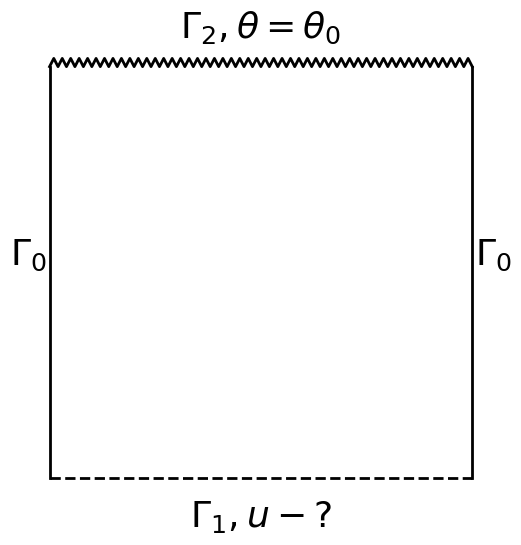
\includegraphics[width=1\linewidth]{omega_1}}
%        \caption*{$\Gamma \coloneqq \partial \Omega =\overline{\Gamma}_0 \cup \overline{\Gamma}_1 \cup \overline{\Gamma}_2$}
    \end{wrapfigure}
    Положим $\Omega = \{(x,y), 0 \leq x,y \leq 1\}$, $l = 1$ см.
    Граница $\partial\Omega$:
    \[
        \begin{aligned}
            \Gamma_0 & = \{x=\{0,1\}, y \in [0,1]\} \\
            \Gamma_1 & = \{x\in [0,1], y=0\}
            - \text{участок с неизвестными отр. свойствами}, \\
            \Gamma_2 & = \{x \in [0,1], y=1\} - \text{участок наблюдения}.
        \end{aligned}
    \]
    Будем также далее считать, что $a = 0.006[\text{см}^2/\text{c}]$,
    $b=0.025[\text{см}/\text{с}]$, $\beta = 0.00005[\text{см}/\text{с}]$,
    $\kappa=1[\text{см}^{-1}]$, $\kappa_s = 0$, $A = 0$, $\gamma = 0.3$.
    Температуру на границе $\Omega$ положим равной $\theta_b = (x^2+y^2)/3$.

    При указанных параметрах для первого эксперимента выберем следующее тестовое
    значение функции $u$:
    \begin{equation*}
        u(x)=
        \begin{cases}
            0.01, & \text{если } x \le 0.5, \\
            0.5, & \text{если } x > 0.5,
        \end{cases}
    \end{equation*}
    и для второго эксперимента:
    $u(x)=0.49x+0.01$.
\end{frame}
\note{
    Положим параметры среды, соответствующие стеклу и зададим тестовую функцию управления
    как показано на слайде.
    Пластинка, у которого боковые стороны "обычные", верхняя грань - участок наблюдения,
    нижняя грань - участок под "контролем".
}


\begin{frame}
    \textbf{Результаты моделирования:}

    \centering
    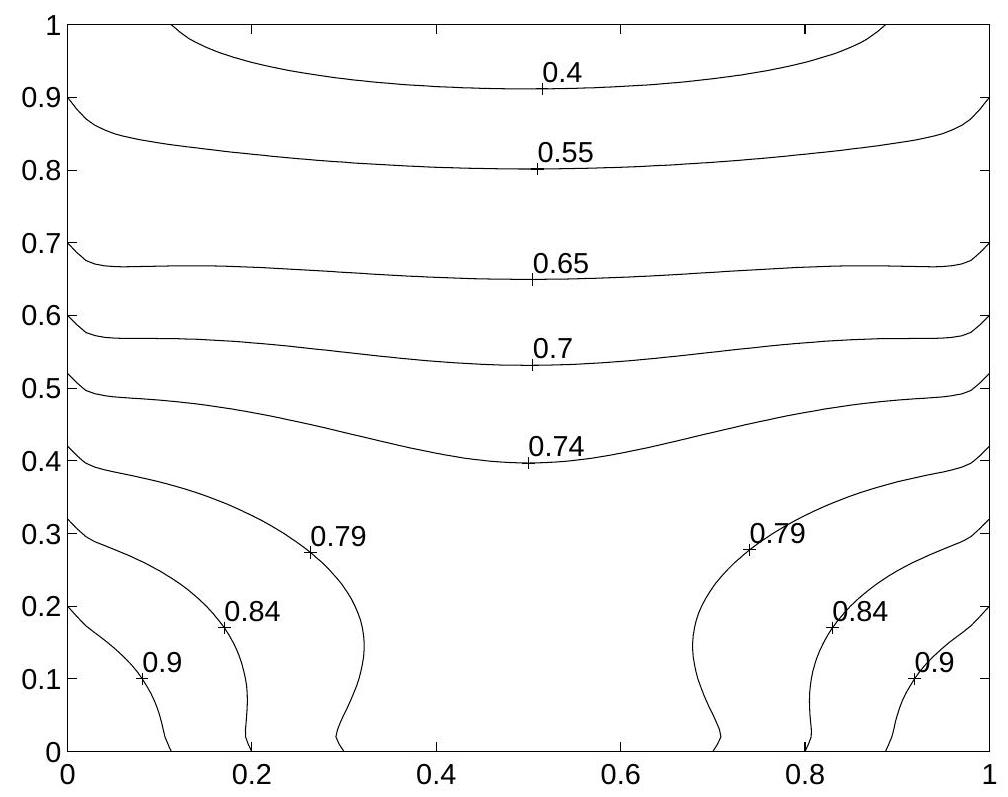
\includegraphics[width=0.42\linewidth]{dvmg368/1}
    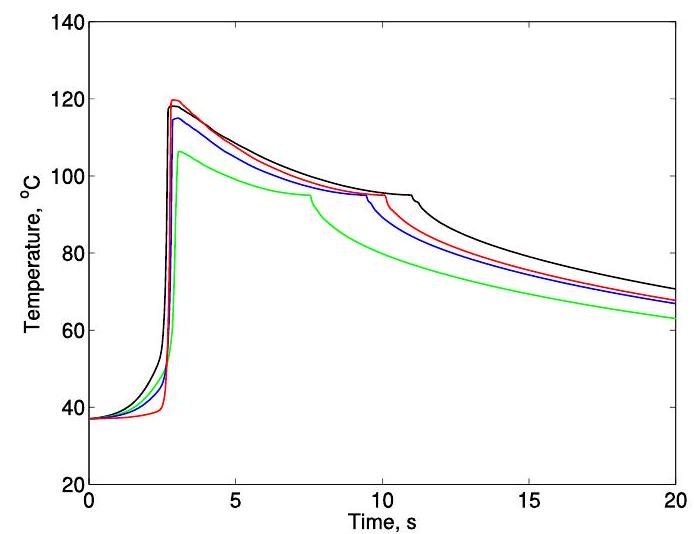
\includegraphics[width=0.42\linewidth]{dvmg368/2}
    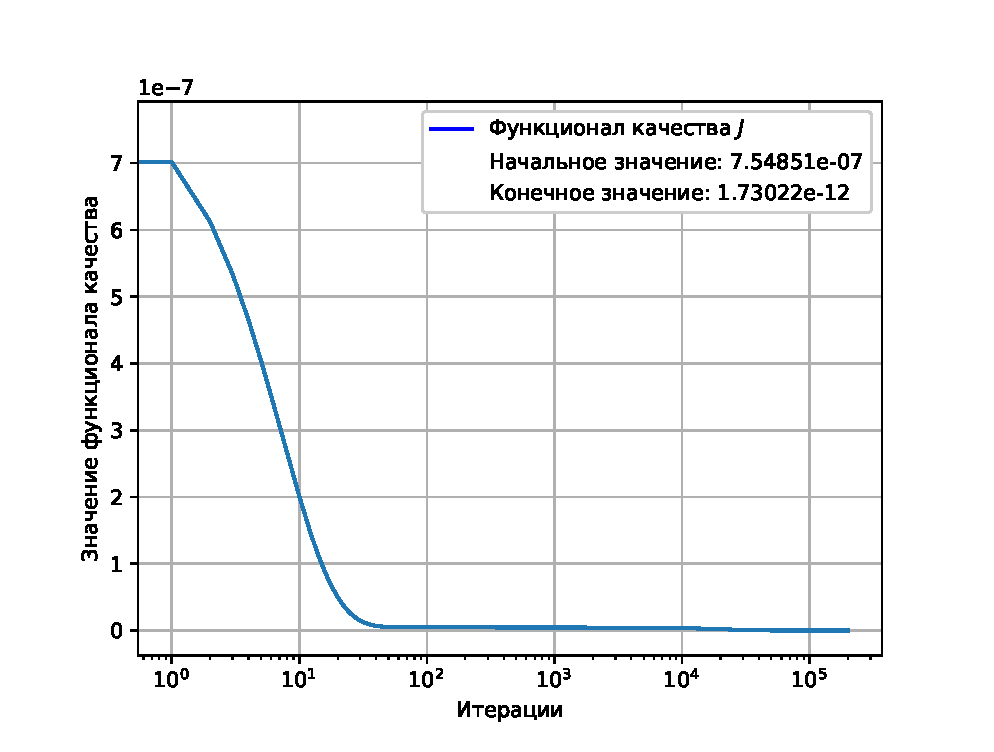
\includegraphics[width=0.42\linewidth]{dvmg368/3}
    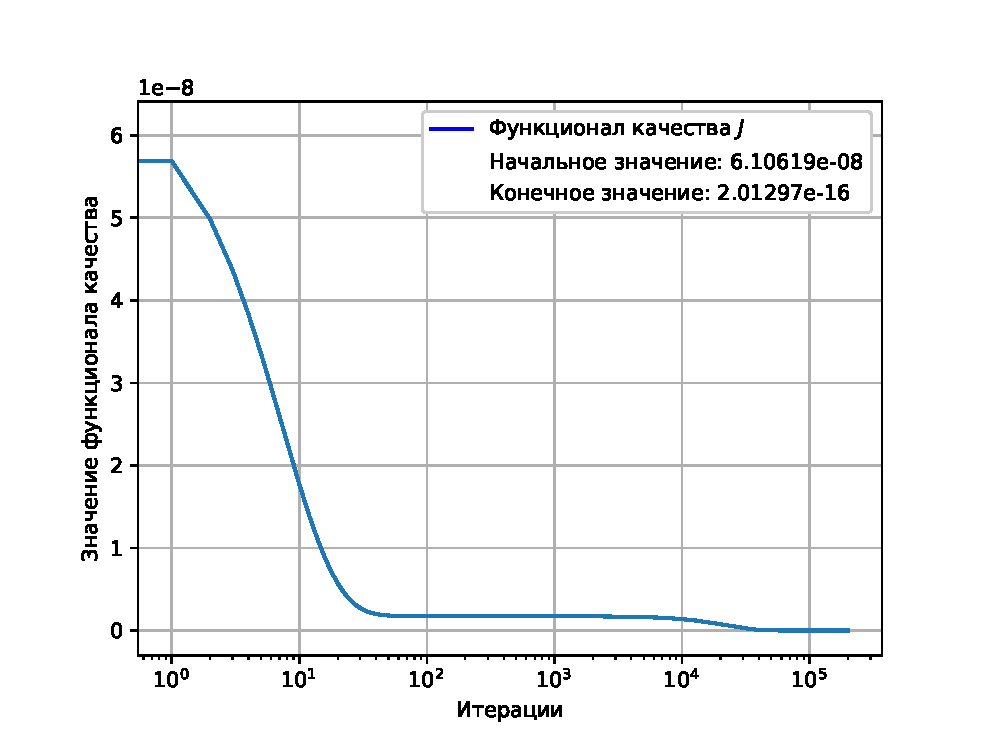
\includegraphics[width=0.42\linewidth]{dvmg368/4}
\end{frame}
\note{
    Интересный эффект "среднего значения". Большое количество итераций.
    Обратить внимание на функционал качества.
    Для получения представленных результатов, использовался разработанный мной комплекс программ,
    включающий решение прямой задачи, сопряженной системы и алгоритм градиентного спуска.
}

\subsection{Обратная задача с условиями типа Коши}\label{subsec:rev_koshi}
\begin{frame}
    \frametitle{Задача без краевых условий для интенсивности излучения}
    \textbf{Краевая задача:}
    \begin{equation}
        \label{eq:2_2:eq1}
        - a \Delta \theta + b \kappa_a(\theta ^ 3 | \theta | - \varphi) = 0,  \quad
        - \alpha \Delta \varphi + \kappa_a (\varphi - \theta ^3 | \theta |) = 0,
    \end{equation}
    На $\Gamma$ известно температурное поле и тепловой поток:
    \begin{equation}
        \label{eq:2_2:bc2} \theta = \theta_b, \quad \partial_n\theta = q_b.
    \end{equation}
    Заменяем на <<искусственные>> краевые условия
    \begin{equation}
        \label{eq:2_2:bc3}
        a(\partial_n\theta+\theta) = r,\;\;
        \alpha(\partial_n\varphi+\varphi) = u \text{ на }\Gamma.
    \end{equation}
    Функция $r(x),\, x\in\Gamma$ является заданной, функция $u(x),\, x\in\Gamma$
    описывающая излучающие свойства участка границы, неизвестна.
    Получаем \textbf{обратную задачу}.

    \textbf{Задача оптимального управления} заключается в отыскании тройки
    $\{\theta_\lambda,\varphi_\lambda,u_\lambda\}$ такой, что
    \begin{equation}
        \label{eq:2_2:cost}
        J_\lambda(\theta, u) = \frac{1}{2}\int\limits_\Gamma (\theta - \theta_b)^2 d\Gamma
        + \frac{\lambda}{2}\int\limits_\Gamma u^2 d\Gamma \rightarrow\inf
    \end{equation}
    на решениях краевой задачи, функция $u(x) x \in \Gamma$ играет роль управления.

    \begin{itemize}
        \item $(j) \;\; a,b,\alpha,\kappa_a, \lambda ={\textrm Const}> 0,$
        \item $(jj) \;\, \theta_b, \,q_b \in U,\;\; r=a(\theta_b+q_b)$.
    \end{itemize}
    \begin{theorem}[2.5]
        \label{th:2_2:3}
        Пусть выполняются условия $(j),(jj)$ и существует решение
        задачи~\eqref{eq:2_2:eq1}--\eqref{eq:2_2:bc2}.
        Если $\{\theta_\lambda,\varphi_\lambda,u_\lambda\}$ -- решение
        задачи оптимального управления для $\lambda>0$, то существует последовательность $\lambda\to +0$
        такая, что
        $\theta_\lambda\rightarrow\theta_*, \;\; \varphi_\lambda\rightarrow\varphi_*
        \text{ слабо в }V,\text{ сильно в }H$,
        где $\theta_*,\varphi_*$ -- решение задачи~\eqref{eq:2_2:eq1}--\eqref{eq:2_2:bc2}.
    \end{theorem}
\end{frame}
\note{
    23. Не задано $\varphi$!
    В основе разработанного алгоритма решения лежит анализ экстремальной задачи.

    Строго обосновано существование решения экстр задачи.
    Кроме того, и это принципиально важно, показана сходимость решений экстремальных задач
    к решению задачи~\eqref{eq:2_2:eq1}--\eqref{eq:2_2:eq2}
    без краевых условий для интенс излучения при $\lambda$ стремящемся к 0.
}
\begin{frame}
    \textbf{Разрешимость задачи оптимального управления и условия оптимальности}

    \begin{theorem}[2.3]
        \label{th:2_2:1}
        Пусть выполняются условия $(j), (jj)$.
        Тогда существует решение задачи $CP$.
    \end{theorem}
    \begin{theorem}[2.4]
        \label{th:2_2:2}
        Пусть выполняются условия $(j),(jj)$.
        Если $\{\hat{\theta}, \hat{\varphi}, \hat{u}\}$ -- решение задачи оптимального управления,
        то существует единственная пара $\{p_1, p_2 \} \in V\times V$ такая, что
        \begin{equation}
            \label{eq:2_2:as}
            aAp_1 +4|\hat{\theta}|^3 \kappa_a(bp_1 - p_2) = B(\theta_b - \hat{\theta}), \;\;
            \alpha A p_2 + \kappa_a (p_2 - b p_1)=0
        \end{equation}
        и при этом $\lambda\hat{u} = p_2$.
    \end{theorem}


    \textbf{Алгоритм решения задачи без краевых условий для интенсивности излучения}

    1.\ Выбираем значение градиентного шага $\varepsilon$,

    2.\ Выбираем количество итераций $N$,

    3.\ Выбираем начальное приближение для управления $u_{0} \in U$,

    4.\ для $k \leftarrow 0,1,2, \ldots, N$ выполнить:

    \hspace{1cm} a.\ Для заданного $u_{k}$, вычислить состояние
    $y_{k}=\left\{\theta_{k}, \varphi_{k}\right\}$, решение
    задачи~\eqref{eq:2_2:eq1}--\eqref{eq:2_2:bc1}.

    \hspace{1cm} b.\ Вычислить значение функционала качества
    $J_{\lambda}\left(\theta_{k}, u_{k}\right)$.

    \hspace{1cm} c.\ Из уравнений~\eqref{eq:2_2:as}, вычислить сопряженное
    состояние $p_{k}=\left\{p_{1k}, p_{2k}\right\}$,
    где $\widehat{\theta} \coloneqq \theta_{k}, \widehat{u} \coloneqq u_{k}$.

    \hspace{1cm} d.\ Пересчитать управление
    $u_{k+1}=u_{k}-\varepsilon\left(\lambda u_{k}-p_{2}\right)$.


    Значение параметра $\varepsilon$ выбирается эмпирически.
    Количество итераций $N$ выбирается достаточным для выполнения условия
    $J_\lambda(\theta_k, u_k) - J_\lambda(\theta_{k+1}, u_{k+1}) < \delta$, где $\delta>0$
    определяет точность расчетов.
\end{frame}
\note{
    25. Условия оптимальности лежат в основе численного метода
}

\begin{frame}
    \textbf{Пример 1.}
    Приведем примеры расчетов для куба $\Omega = {(x, y, z), 0 \leq x,y,z \leq l}$.

    Будем считать, что $l=1~\text{см}$, $a = 0.006[\text{см}^2/\text{c}]$,
    $b=0.025[\text{см}/\text{с}]$, $\kappa_a=1[\text{см}^{-1}]$, $\alpha = 0.(3)[\text{см}]$.
    Параметр регуляризации $\lambda=10^{-12}$.

    Определим $r$ и $u$ в~\eqref{eq:2_2:bc3} как $r = 0.7, \quad u = \hat u = 0.5$.
    Для обозначенных параметров рассчитаем функции $\theta$, $\varphi$ из решения граничной задачи
    и положим $\theta_b = \theta|_\Gamma$.
    Нормальная производная $\partial_n \theta = q_b = r / a - \theta_b$.

    Применяя алгоритм градиентного спуска найдем решение задачи оптимального управления.
    \begin{figure}[h!t]
        \begin{minipage}[b][][b]{0.49\linewidth}
            \centering
            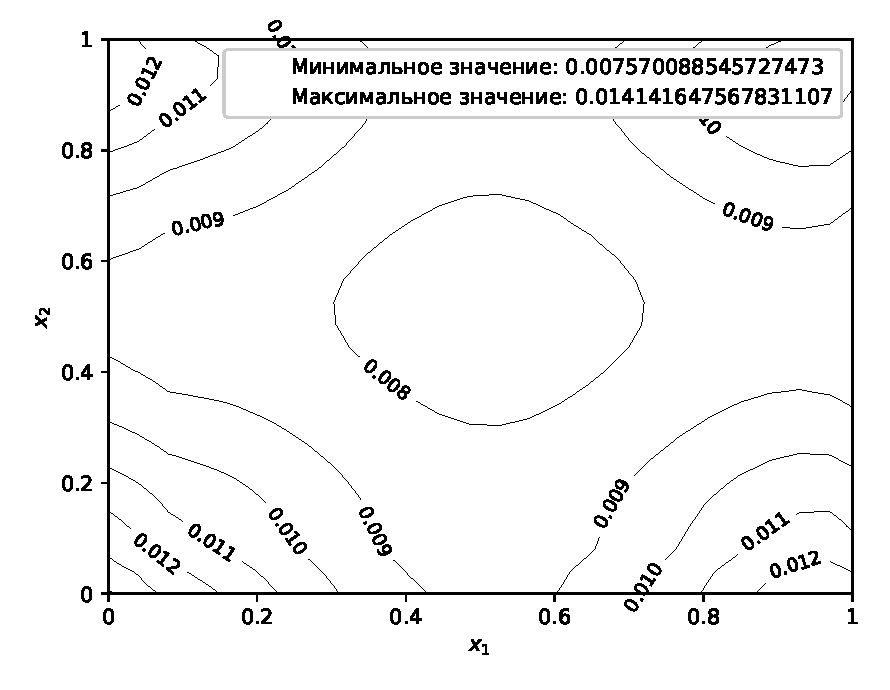
\includegraphics[width=1\linewidth]{jvm-2020/exp1/theta_n_diff_iso}
            \\ а) $|\partial_n\theta_\lambda-q_b|/|q_b|$
        \end{minipage}
        \hfill
        \begin{minipage}[b][][b]{0.49\linewidth}
            \centering
            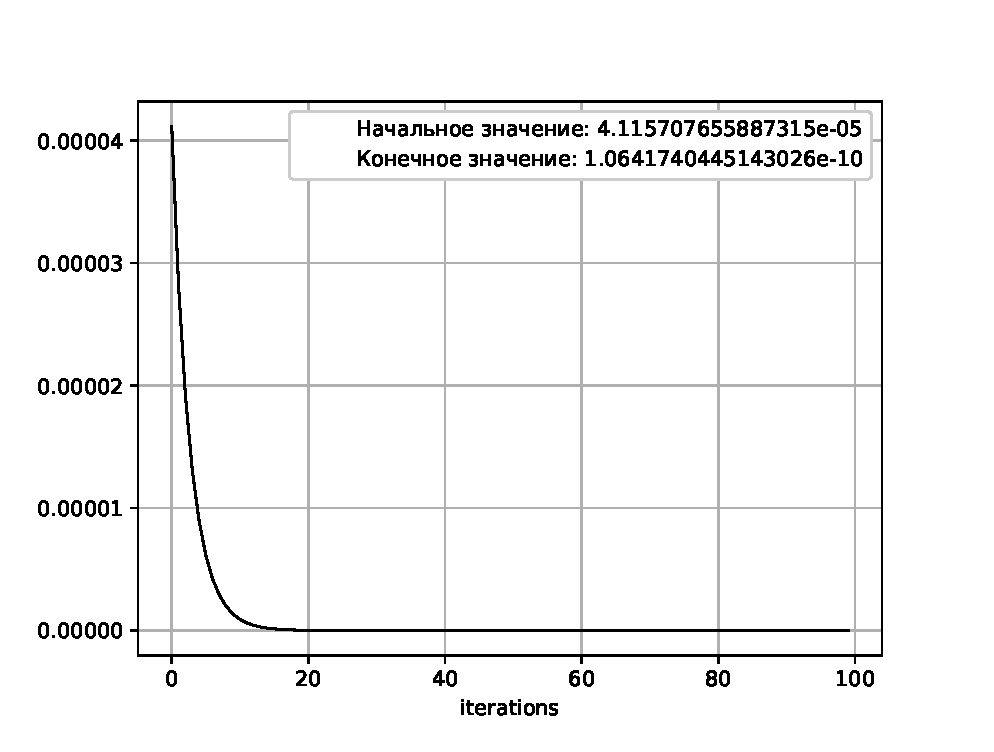
\includegraphics[width=1\linewidth]{jvm-2020/exp1/quality}
            \\ б) Значение функционала качества
        \end{minipage}
        \label{fig:4_4:0}
    \end{figure}
\end{frame}
\note{
    Обратите внимание на малость функционала качества.
    Сравним с тем, что получилось -- довольно близко, но не идеально.
    Уменьшение параметра регуляризации повышает точность решения,
    но и увеличивает вычислительные затраты.
}

\begin{frame}
    \textbf{Пример 2.}


    Зададим функции $\theta_{b}, q_{b}$ в краевом условии~\eqref{eq:2_2:bc2}
    следующим образом:
    \[
        \theta_{b}=0.1 z+0.3, \quad q_{b}=
        \begin{cases}
            0.11, & \text { если } z=1, \\
            0, & \text { если } 0<z<1, \\
            -0.15, & \text { если } z=0.
        \end{cases}
    \]

    В данном примере оптимальное управление $u$ в качестве тестового не задается.
    Начальное значение функционала качества $J_\lambda$ составляет $7.20 \cdot 10^{-6}$.
    Финальное значение $2.86 \cdot 10^{-10}$.

    \begin{figure}[h!t]
        \begin{minipage}[b][][b]{0.49\linewidth}
            \centering
            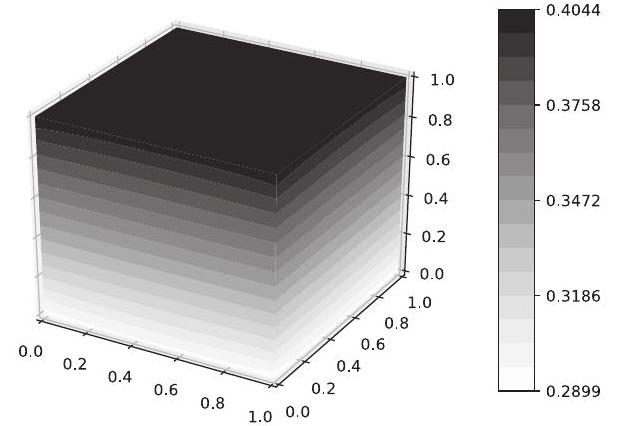
\includegraphics[width=0.9\linewidth]{jvm-2020/dvmg/3b}
            \\ а) Полученное температурное поле $\theta_\lambda$
        \end{minipage}
        \hfill
        \begin{minipage}[b][][b]{0.49\linewidth}
            \centering
            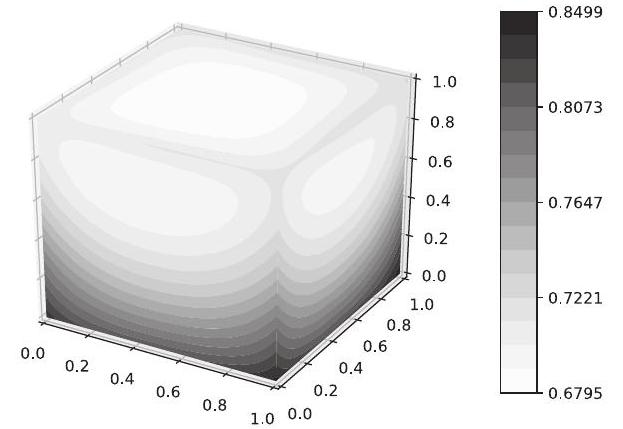
\includegraphics[width=1\linewidth]{jvm-2020/dvmg/2a}
            \\ б) Полученное поле излучения $\varphi_\lambda$
        \end{minipage}
        \label{fig:4_4:3}
    \end{figure}

\end{frame}
\note{
    "Честный" эксперимент - используем то, что полагается в исходной задаче.
    Функционал качества (его динамика) позволяет предположить аналогичный порядок
    близости (с предыдущим примером)
    точного и аппроксимированного решений.
    Обратите внимание на линейность $\theta_b$ по оси $z$.
}
